\chapter{States, Measurements, and Complex Vector Spaces}

\lectureoverview{Quantum mechanics begins by changing what we mean by a state. We first isolate the classical pattern of states and deterministic updating, then use a two-outcome spin experiment to expose its failure. The mathematical response is a complex vector space equipped with dual vectors, an inner product, a norm, and orthogonality.}

\section{The Classical Pattern: State and Update}

Begin with a closed system, at least temporarily isolated from everything else. The word \emph{system} is primitive here: it means the object whose history we want to predict. A \emph{state} is everything that must be known at one instant in order to make that prediction. Classical mechanics supplies a law that updates one state into the next.

For the simplest abstract coin,
\begin{equation}
  \mathcal S_{\mathrm{coin}}=\{H,T\}.
\end{equation}
One possible law says that nothing happens:
\begin{equation}
  H\longmapsto H,
  \qquad
  T\longmapsto T.
\end{equation}
Another law alternates the two states:
\begin{equation}
  H\longmapsto T,
  \qquad
  T\longmapsto H.
\end{equation}
These examples are elementary, but they expose the architecture of a classical theory:
\begin{equation}
  s(t)\longmapsto s(t+\Delta t).
\end{equation}
Once \(s(t)\) is known, the update is deterministic.

The same pattern survives when the state space is continuous. A particle moving on a line requires both its position and momentum,
\begin{equation}
  s=(q,p),
\end{equation}
so its state space is the phase plane. The number of possible states has become infinite, and the equations may be written in the elegant language of Lagrangians, Hamiltonians, and Poisson brackets, but the underlying idea has not changed. The state at one time contains what is needed to predict the state at another.

\section{Abstraction Before Visualization}

Classical motion is comparatively easy to picture because its concepts are drawn from ordinary experience. That advantage disappears when the relevant objects are too small, the velocities too large, or the dimension of the state space too high. No one literally visualizes the motion of an electron, four-dimensional spacetime, or a ten-dimensional space. This is not a deficiency peculiar to beginners. Human visual intuition was built for the everyday three-dimensional world.

Even apparently simpler cases reveal the limitation. What we call a picture of a two-dimensional curved space is ordinarily a surface embedded in three dimensions. A one-dimensional line is pictured as a mark in a plane. The picture quietly imports the ambient space in which our visual system knows how to operate.

The remedy is not to force a classical picture onto unfamiliar physics. It is to learn the abstract structure and let a new intuition grow from correct manipulations. Three-dimensional coordinates \((x,y,z)\) become four-dimensional coordinates \((x,y,z,w)\) by adding a symbol and extending the rules, not by acquiring a new organ of sight. Quantum mechanics demands the same discipline. Treating it as a strange mechanical model of little classical objects will repeatedly produce the wrong answer.

\begin{remark}
Mathematical intuition still develops. It is simply not the same as seeing a wave on the ocean or an arrow in ordinary space. The algebra becomes familiar because its relations are used consistently.
\end{remark}

\section{Classical State Spaces and Classical Logic}

For a classical system, the state space is a set. An abstract die has
\begin{equation}
  \mathcal S_{\mathrm{die}}=\{1,2,3,4,5,6\}.
\end{equation}
A real die has continuously many orientations, but the idealized die used here has only these six labels. A particle on a line has the continuously infinite set
\begin{equation}
  \mathcal S_{\mathrm{particle}}
  =
  \{(q,p)\mid q,p\in\mathbb R\}.
\end{equation}
Finite or infinite, each classical state space is a collection of mutually distinct possibilities.

A proposition about the system selects a subset of those possibilities. For the die, let
\begin{align}
  P_{\mathrm{odd}}&=\{1,3,5\},\\
  P_{\leq 3}&=\{1,2,3\}.
\end{align}
The statement \emph{odd and no greater than three} corresponds to their intersection:
\begin{equation}
  P_{\mathrm{odd}}\cap P_{\leq 3}=\{1,3\}.
\end{equation}
The inclusive statement \emph{odd or no greater than three} corresponds to their union:
\begin{equation}
  P_{\mathrm{odd}}\cup P_{\leq 3}
  =
  \{1,2,3,5\}.
\end{equation}
Thus classical conjunction and disjunction have the set-theoretic form
\begin{equation}
  P\wedge Q\longleftrightarrow P\cap Q,
  \qquad
  P\vee Q\longleftrightarrow P\cup Q.
\end{equation}
If the subsets do not overlap, no state makes both propositions true.

This logic is tied to the classical conception of state. Quantum mechanics replaces the set of classical alternatives by a different mathematical object: a vector space. Only in a suitable classical limit does the vector-space description behave approximately like a set of exclusive configurations. Before constructing that space, we need an experiment that makes the replacement unavoidable.

\section{The Simplest Quantum System}

The quantum analogue of the abstract coin is a two-outcome system called a \emph{qubit}. Its measured alternatives may first be labeled heads and tails, but a numerical label is more useful:
\begin{equation}
  \sigma\in\{+1,-1\}.
\end{equation}
Three notations will be used in parallel:
\begin{equation}
  H\longleftrightarrow \sigma=+1\longleftrightarrow\uparrow,
  \qquad
  T\longleftrightarrow \sigma=-1\longleftrightarrow\downarrow.
\end{equation}
At first the arrows are only names. No ordinary geometric vector has yet been assumed.

\begin{figure}[htbp]
  \centering
  
\includegraphics[width=0.78\textwidth]{lecture_01_figure_02.png}
  \caption{The board introduces the equivalent labels \(H/T\), \(\sigma=\pm1\), and up/down arrows. The arrows begin as notation, not as a classical model.}
  \lectureframe{00:22:44}
\end{figure}

\begin{classroomqa}
\audiencequestion{What do heads and tails have to do with the physical system?}
\lecturerresponse{Nothing beyond providing two familiar names. The qubit has two possible outcomes for this measurement; heads and tails are placeholders. The labels \(\pm1\) are chosen because they can enter equations.}
\end{classroomqa}

\subsection{The Apparatus as a Black Box}

An experiment requires a second system, the apparatus \(A\). For now it is an abstract black box with three features:
\begin{enumerate}
  \item it has a spatial orientation, marked by \emph{this side up};
  \item it has a sensor that can interact with the qubit;
  \item it has a display that is initially blank and afterward reads \(+1\) or \(-1\).
\end{enumerate}
The details of the detector are deliberately postponed. A good detector is defined operationally by the reliable relation between the system and its record. The observer need not be watching when the interaction occurs; the apparatus can record the result and be read later.

Suppose the display reports \(+1\). Reset the apparatus to its blank condition and repeat the same measurement immediately, before any independent evolution has time to act. A faithful detector reports \(+1\) again. If the first result is \(-1\), immediate repetitions likewise continue to report \(-1\):
\begin{equation}
\begin{aligned}
  +1&\longrightarrow +1\longrightarrow +1\longrightarrow\cdots,\\
  -1&\longrightarrow -1\longrightarrow -1\longrightarrow\cdots.
\end{aligned}
\end{equation}
The first measurement can therefore be regarded as a \emph{preparation}. It leaves the qubit in a state for which an immediate repetition of the same measurement has a definite result.

This repeatability is not an optional philosophical gloss. Without it there would be no operational way to confirm a measurement. A defective device may fail to repeat its result, but then it is not carrying out the ideal measurement being defined.

\begin{classroomqa}
\audiencequestion{Is this already the collapse of the wave function?}
\lecturerresponse{That language can be introduced later. At this stage the operational statement is enough: a measurement produces a result and prepares a state in which the same immediate measurement reproduces that result. Naming the process does not yet explain it.}
\end{classroomqa}

\section{Orientation and the Failure of the Classical Pointer}

Prepare the qubit so that the upright apparatus reads \(+1\). Turn the apparatus through \(180^\circ\) and repeat the measurement. The result is now \(-1\). Repeated measurements with the inverted apparatus confirm \(-1\), while turning the apparatus upright again restores \(+1\).

The result reveals genuine directionality. The up/down notation is not entirely arbitrary: reversing the detector reverses the sign. It is tempting to conclude that the qubit is simply a small vector and that the detector measures the component of that vector along its own axis. That temptation must be tested rather than trusted.

\begin{figure}[htbp]
  \centering
  
\includegraphics[width=0.82\textwidth]{lecture_01_figure_03.png}
  \caption{An upward preparation and differently oriented analyzers on the board. The classroom later corrected the direction of one chalk arrow; only the analyzer axis matters in the argument.}
  \lectureframe{00:36:21}
\end{figure}

\subsection{A Sideways Measurement}

Turn the detector by \(90^\circ\). If the prepared qubit were an ordinary upward pointer, its component along the horizontal detector axis would be zero:
\begin{equation}
  \hat{\mathbf x}\cdot\hat{\mathbf z}=0.
\end{equation}
The quantum apparatus never reports zero. Every individual trial reports either \(+1\) or \(-1\).

\begin{figure}[htbp]
  \centering
  \resizebox{\linewidth}{!}{%
  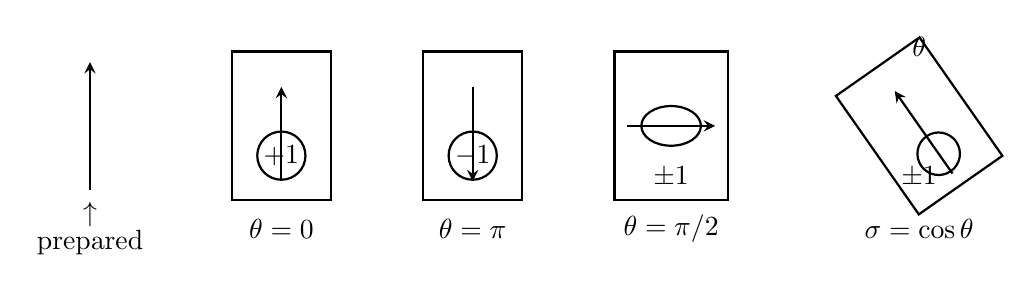
\begin{tikzpicture}[>=stealth,thick,scale=0.90]
    \draw[->] (0,0)--(0,1.8);
    \node at (0,-0.35) {\(\uparrow\)};
    \node at (0,-0.75) {prepared};

    \draw (2.0,-0.15) rectangle (3.4,1.95);
    \draw (2.7,0.48) circle (0.34);
    \draw[->] (2.7,0.12)--(2.7,1.45);
    \node at (2.7,0.48) {\(+1\)};
    \node at (2.7,-0.55) {\(\theta=0\)};

    \draw (4.7,-0.15) rectangle (6.1,1.95);
    \draw (5.4,0.48) circle (0.34);
    \draw[->] (5.4,1.45)--(5.4,0.12);
    \node at (5.4,0.48) {\(-1\)};
    \node at (5.4,-0.55) {\(\theta=\pi\)};

    \draw (7.4,-0.15) rectangle (9.0,1.95);
    \draw (8.2,0.90) ellipse (0.42 and 0.28);
    \draw[->] (7.58,0.90)--(8.82,0.90);
    \node at (8.2,0.18) {\(\pm1\)};
    \node at (8.2,-0.55) {\(\theta=\pi/2\)};

    \begin{scope}[shift={(11.7,0.90)},rotate=35]
      \draw (-0.72,-1.02) rectangle (0.72,1.02);
      \draw (0,-0.48) circle (0.30);
      \draw[->] (0,-0.82)--(0,0.60);
    \end{scope}
    \node at (11.7,0.18) {\(\pm1\)};
    \node at (11.7,-0.55) {\(\expect{\sigma}=\cos\theta\)};
    \node at (11.7,2.02) {\(\theta\)};
  \end{tikzpicture}
  }%
  \caption{Reconstruction of the analyzer sequence. A rotation changes the statistics, never the set of individual outcomes.}
\end{figure}

Prepare a large collection of qubits with the upright apparatus, retaining those for which the result is \(+1\). Measure each retained qubit once with the sideways apparatus. Half the trials give \(+1\), half give \(-1\), and the ensemble average is zero:
\begin{equation}
  \expect{\sigma}_{\pi/2}=0.
\end{equation}
The average resembles the vanishing horizontal component of a classical pointer, but the individual records do not. The classical value \(0\) has been replaced by a statistical balance between two discrete outcomes.

\begin{classroomqa}
\audiencequestion{What happens if the same qubit is kept instead of being discarded after the sideways measurement?}
\lecturerresponse{Suppose its first sideways result is \(+1\). Repeating the sideways measurement on that same qubit gives \(+1\) again and again. The first sideways measurement has prepared it relative to the sideways axis. To obtain the fifty-fifty statistics, one must repeat the whole preparation-and-measurement experiment on many qubits, not repeatedly confirm one result.}
\end{classroomqa}

\subsection{Incompatible Preparations}

The sequence of axes matters. Prepare \(+1\) vertically, then measure horizontally. The first horizontal result is random. Once a horizontal result has been obtained, immediate horizontal repetitions are definite. Now turn the detector back to the vertical axis. The vertical result is random again.

In symbols, where \(M_z\) and \(M_x\) denote measurements along the two axes,
\begin{equation}
\begin{aligned}
  M_z&:+1,\\
  M_x&:\pm1,\\
  M_x&:\text{same result},\\
  M_z&:\pm1.
\end{aligned}
\end{equation}
The intermediate \(x\)-measurement has not merely uncovered a horizontal component while preserving the original vertical state. It has prepared a new state, and the original vertical definiteness is gone.

\begin{classroomqa}
\audiencequestion{Does the detector remember the first answer? How can it know whether the same qubit or a new qubit has been presented?}
\lecturerresponse{The repeatability is a property of the measured qubit, not a hidden memory comparison performed by the detector. After a measurement, the qubit is in a state that gives the same answer to the same immediate measurement. Present a differently prepared qubit and the result depends on that preparation. Keeping track of which physical system is being measured is ordinary laboratory bookkeeping.}
\end{classroomqa}

\begin{classroomqa}
\audiencequestion{So the act of observing prepares the particular qubit?}
\lecturerresponse{Yes. Once that measurement has prepared the qubit, the same measurement gives the same answer until some other evolution or incompatible measurement intervenes.}
\end{classroomqa}

\section{An Arbitrarily Rotated Analyzer}

Let the detector axis make an angle \(\theta\) with the axis along which the ensemble was prepared. Every trial still yields
\begin{equation}
  \sigma=\pm1.
\end{equation}
The relative frequencies vary with the angle so that the mean is
\begin{equation}
  \expect{\sigma}_{\theta}=\cos\theta.
  \label{eq:qml1-cosine-mean}
\end{equation}
The limiting cases are
\begin{align}
  \expect{\sigma}_{0}&=+1,\\
  \expect{\sigma}_{\pi/2}&=0,\\
  \expect{\sigma}_{\pi}&=-1.
\end{align}
Near \(\theta=0\), most outcomes are \(+1\), with an occasional \(-1\). Near \(\theta=\pi\), most are \(-1\), with an occasional \(+1\).

\begin{figure}[htbp]
  \centering
  
\includegraphics[width=0.82\textwidth]{lecture_01_figure_04.png}
  \caption{The actual board for the arbitrary-angle experiment: a vertically prepared ensemble enters an analyzer tilted by \(\theta\).}
  \lectureframe{00:48:55}
\end{figure}

The smooth vector-like quantity is the ensemble mean, not the single result. If \(p_+(\theta)\) and \(p_-(\theta)\) are the two probabilities, then
\begin{equation}
  p_+ + p_-=1,
  \qquad
  p_+-p_-=\cos\theta.
\end{equation}
Consequently,
\begin{equation}
\begin{aligned}
  p_+(\theta)&=\frac{1+\cos\theta}{2}
  =\cos^2\frac{\theta}{2},\\
  p_-(\theta)&=\frac{1-\cos\theta}{2}
  =\sin^2\frac{\theta}{2}.
\end{aligned}
  \label{eq:qml1-half-angle-probabilities}
\end{equation}
\editorialnote{The lecture states the two outcomes and their mean \(\cos\theta\). Equation~\eqref{eq:qml1-half-angle-probabilities} is the immediate algebraic consequence of those statements and makes the implied frequency law explicit.}

\begin{classroomqa}
\audiencequestion{Would an unprepared collection of qubits also show the \(\cos\theta\) mean?}
\lecturerresponse{No particular direction has been selected in an unpolarized collection, so its mean is zero. The \(\theta\)-dependence refers to an ensemble first prepared along a definite axis.}
\end{classroomqa}

\begin{classroomqa}
\audiencequestion{Why is a whole ensemble necessary if the qubit has no intervening dynamics?}
\lecturerresponse{The first tilted measurement on one qubit gives one sample. Every immediate repetition on that same qubit only confirms that sample. Independent trials require identically prepared qubits, each measured once with the tilted analyzer.}
\end{classroomqa}

\begin{classroomqa}
\audiencequestion{Are there patterns or higher-order correlations in the sequence of pluses and minuses?}
\lecturerresponse{For this experiment the separate trials are taken to be independent and uncorrelated. Their one-trial probabilities depend on \(\theta\), but no additional ordering pattern is being asserted.}
\end{classroomqa}

\subsection{What Has Been Idealized}

For the moment the apparatus is treated as a classical object with a continuously adjustable orientation and a discrete readout. This division between \emph{system} and \emph{detector} is temporary. The detector is itself a physical system and must eventually obey quantum mechanics. A complete account will treat system and apparatus together, but that requires machinery not yet available.

\begin{classroomqa}
\audiencequestion{Is the detector itself just another two-state system?}
\lecturerresponse{It has physical states and must ultimately be included in the quantum description. For now we retain an operational split: the qubit is the object being described quantum mechanically, while the oriented detector supplies a stable classical record. Later the combined system must be analyzed as interacting quantum systems.}
\end{classroomqa}

\begin{classroomqa}
\audiencequestion{Does changing the axis about which the detector is rotated introduce more structure than the single angle shown here?}
\lecturerresponse{Yes, the full three-dimensional story is richer. The one-plane rotation is the simplest slice of it and is consistent with the more complete treatment to come.}
\end{classroomqa}

\begin{classroomqa}
\audiencequestion{Can the detector return a continuous value between \(-1\) and \(+1\)?}
\lecturerresponse{Its orientation varies continuously, but each ideal qubit readout remains \(+1\) or \(-1\). Continuity appears in the probabilities and averages as the orientation changes, not in the individual outcomes.}
\end{classroomqa}

\section{Pointers and Abstract Vectors}

The experimental facts are now separated from the mathematics for a while. An ordinary arrow in physical space will be called a \emph{pointer}. A mathematical vector is more general: it is an element of a vector space and need not point anywhere in ordinary space.

\begin{definition}
A complex vector space \(V\) is a collection of vectors for which vector addition and multiplication by complex scalars are defined and satisfy the usual linearity rules. In particular, for \(u,v,w\in V\) and \(a,b\in\mathbb C\),
\begin{align}
  u+v&=v+u,\\
  (u+v)+w&=u+(v+w),\\
  a(u+v)&=au+av,\\
  (a+b)u&=au+bu,\\
  (ab)u&=a(bu),\\
  1u&=u.
\end{align}
There is a zero vector \(0\) and an additive inverse \(-u\) for every \(u\).
\end{definition}

The classroom discussion initially emphasizes only the operations and closure:
\begin{equation}
\begin{aligned}
  u,v\in V&\Longrightarrow u+v\in V,\\
  a\in\mathbb C,\ u\in V&\Longrightarrow au\in V.
\end{aligned}
\end{equation}
The zero vector and commutativity are then supplied in response to questions. The remaining familiar axioms state explicitly what is already used when the concrete column-vector model is introduced.

Real numbers form a one-dimensional vector space over \(\mathbb R\). Complex numbers form a one-dimensional vector space over \(\mathbb C\), and a two-dimensional vector space over \(\mathbb R\). Complex-valued functions \(\psi(x)\) also form a complex vector space because
\begin{equation}
  (\psi+\phi)(x)=\psi(x)+\phi(x),
  \qquad
  (z\psi)(x)=z\psi(x).
\end{equation}
This function-space example will later become central, but finite columns make the structure easier to see first.

\begin{classroomqa}
\audiencequestion{What is the distinction between a vector and a vector space?}
\lecturerresponse{A vector is one element. A vector space is the collection of all such elements together with the rules for adding them and multiplying them by scalars, just as a number is one object while the number system is a collection with operations.}
\end{classroomqa}

\section{Two-Component Complex Columns}

Write an abstract vector in Dirac notation as \(\ket{\alpha}\). A concrete representation is
\begin{equation}
  \ket{\alpha}
  \longleftrightarrow
  \begin{pmatrix}
    \alpha_1\\
    \alpha_2
  \end{pmatrix},
  \qquad
  \alpha_1,\alpha_2\in\mathbb C.
\end{equation}
If
\begin{equation}
  \ket{\beta}
  \longleftrightarrow
  \begin{pmatrix}
    \beta_1\\
    \beta_2
  \end{pmatrix},
\end{equation}
then addition and scalar multiplication are defined component by component:
\begin{align}
  \ket{\alpha}+\ket{\beta}
  &\longleftrightarrow
  \begin{pmatrix}
    \alpha_1+\beta_1\\
    \alpha_2+\beta_2
  \end{pmatrix},\\
  z\ket{\alpha}
  &\longleftrightarrow
  \begin{pmatrix}
    z\alpha_1\\
    z\alpha_2
  \end{pmatrix},
  \qquad z\in\mathbb C.
\end{align}

\begin{figure}[htbp]
  \centering
  
\includegraphics[width=0.88\textwidth]{lecture_01_figure_05.png}
  \caption{The component rules for adding two complex columns and multiplying a column by a complex scalar.}
  \lectureframe{01:14:28}
\end{figure}

The zero vector is
\begin{equation}
  \ket{0}
  =
  \begin{pmatrix}
    0\\
    0
  \end{pmatrix},
  \qquad
  \ket{\alpha}+\ket{0}=\ket{\alpha}.
\end{equation}
Columns of length three form another vector space, and similarly for any fixed length. A two-component column cannot be added to a three-component column because the two belong to different spaces and no componentwise rule relates them.

\begin{classroomqa}
\audiencequestion{Is a column vector a matrix?}
\lecturerresponse{In general terminology it is a matrix with one column. In this course, the word \emph{matrix} will usually mean a square array, while a one-column array will be called a column vector. The distinction is terminological, not a disagreement about the algebra.}
\end{classroomqa}

\begin{classroomqa}
\audiencequestion{Does the order of vector addition matter?}
\lecturerresponse{No. Componentwise addition inherits commutativity from complex numbers:
\[
  \ket{\alpha}+\ket{\beta}
  =
  \ket{\beta}+\ket{\alpha}.
\]
This is one of the vector-space axioms.}
\end{classroomqa}

\section{Dual Vectors: Bras and Kets}

For every ket \(\ket{A}\) there is a corresponding vector in the dual space, written \(\bra{A}\). The map from ket to bra is additive but conjugates complex scalars:
\begin{align}
  \ket{A}+\ket{B}
  &\longleftrightarrow
  \bra{A}+\bra{B},\\
  z\ket{A}
  &\longleftrightarrow
  z^*\bra{A}.
  \label{eq:qml1-antilinear-dual}
\end{align}
This second rule is the essential complex feature. The dual of a scalar multiple is multiplied by the complex conjugate scalar.

\begin{figure}[htbp]
  \centering
  
\includegraphics[width=0.86\textwidth]{lecture_01_figure_06.png}
  \caption{The ket-to-bra correspondence and its two rules: sums map to sums, while scalar multiplication is complex conjugated.}
  \lectureframe{01:23:15}
\end{figure}

For the two-component realization,
\begin{equation}
  \ket{\alpha}
  =
  \begin{pmatrix}
    \alpha_1\\
    \alpha_2
  \end{pmatrix}
  \qquad\Longrightarrow\qquad
  \bra{\alpha}
  =
  \begin{pmatrix}
    \alpha_1^*&\alpha_2^*
  \end{pmatrix}.
  \label{eq:qml1-bra-from-ket}
\end{equation}
Complex conjugation implements the dual correspondence, and the row notation keeps the two kinds of object visibly distinct. Equation~\eqref{eq:qml1-bra-from-ket} also verifies Equation~\eqref{eq:qml1-antilinear-dual} directly.

\section{The Inner Product}

Given \(\ket{\alpha}\) and \(\ket{\beta}\), combine the bra associated with \(\beta\) and the ket \(\alpha\):
\begin{equation}
  \braket{\beta}{\alpha}
  =
  \begin{pmatrix}
    \beta_1^*&\beta_2^*
  \end{pmatrix}
  \begin{pmatrix}
    \alpha_1\\
    \alpha_2
  \end{pmatrix}
  =
  \beta_1^*\alpha_1+\beta_2^*\alpha_2.
  \label{eq:qml1-inner-product}
\end{equation}
The word \emph{bracket} is literally assembled from \emph{bra} and \emph{ket}. This is the complex analogue of a dot product: multiply corresponding components and add, with complex conjugation on the bra.

\begin{figure}[htbp]
  \centering
  
\includegraphics[width=0.88\textwidth]{lecture_01_figure_07.png}
  \caption{The board evaluates the inner product \(\braket{\beta}{\alpha}\) as \(\beta_1^*\alpha_1+\beta_2^*\alpha_2\).}
  \lectureframe{01:31:25}
\end{figure}

Interchanging the vectors gives
\begin{equation}
  \braket{\alpha}{\beta}
  =
  \alpha_1^*\beta_1+\alpha_2^*\beta_2
  =
  \braket{\beta}{\alpha}^{*}.
  \label{eq:qml1-conjugate-symmetry}
\end{equation}
The order therefore matters in general, but only by complex conjugation.

\begin{classroomqa}
\audiencequestion{Could one define a product of complex vectors without conjugating one side?}
\lecturerresponse{One can invent such a bilinear expression, but then the product of a vector with itself need not be real or positive. That structure is not the useful one for quantum mechanics. The conjugated, or Hermitian, inner product gives the norm and probability structure that will be needed.}
\end{classroomqa}

\subsection{Norm and Positivity}

Set \(\beta=\alpha\) in Equation~\eqref{eq:qml1-inner-product}:
\begin{equation}
  \braket{\alpha}{\alpha}
  =
  \alpha_1^*\alpha_1+\alpha_2^*\alpha_2
  =
  |\alpha_1|^2+|\alpha_2|^2.
  \label{eq:qml1-norm-square}
\end{equation}
This number equals its own complex conjugate, so it is real. It is nonnegative, and it vanishes only for the zero vector. The length is defined by
\begin{equation}
  \|\alpha\|
  =
  \sqrt{\braket{\alpha}{\alpha}}.
\end{equation}
Complex components therefore produce an ordinary nonnegative real length.

\begin{figure}[htbp]
  \centering
  
\includegraphics[width=0.88\textwidth]{lecture_01_figure_08.png}
  \caption{The self-inner-product on the board: \(\braket{\alpha}{\alpha}=|\alpha_1|^2+|\alpha_2|^2\), the squared norm.}
  \lectureframe{01:34:40}
\end{figure}

\section{Orthogonality and Dimension}

Two vectors are orthogonal when their inner product vanishes:
\begin{equation}
  \braket{\beta}{\alpha}=0.
  \label{eq:qml1-orthogonality}
\end{equation}
Conjugate symmetry makes this relation independent of order:
\begin{equation}
  \braket{\beta}{\alpha}=0
  \quad\Longrightarrow\quad
  \braket{\alpha}{\beta}
  =
  \braket{\beta}{\alpha}^{*}
  =0.
\end{equation}

In the two-component space, the simplest orthogonal pair is
\begin{equation}
  \ket{e_1}
  =
  \begin{pmatrix}
    1\\
    0
  \end{pmatrix},
  \qquad
  \ket{e_2}
  =
  \begin{pmatrix}
    0\\
    1
  \end{pmatrix},
  \qquad
  \braket{e_1}{e_2}=0.
  \label{eq:qml1-standard-basis}
\end{equation}

\begin{figure}[htbp]
  \centering
  
\includegraphics[width=0.88\textwidth]{lecture_01_figure_09.png}
  \caption{The board constructs the standard orthogonal columns \((1,0)^{\mathsf T}\) and \((0,1)^{\mathsf T}\).}
  \lectureframe{01:39:50}
\end{figure}

The dimension can be characterized as the largest number of mutually orthogonal nonzero vectors. In a two-dimensional space there can be two such vectors but no third. To see this concretely, let
\begin{equation}
  \ket{v}
  =
  \begin{pmatrix}
    v_1\\
    v_2
  \end{pmatrix}
\end{equation}
be orthogonal to both vectors in Equation~\eqref{eq:qml1-standard-basis}. Then
\begin{equation}
  \braket{e_1}{v}=v_1=0,
  \qquad
  \braket{e_2}{v}=v_2=0,
\end{equation}
so \(\ket{v}=\ket{0}\). There is no third nonzero vector orthogonal to both.

\begin{classroomqa}
\audiencequestion{Is not the zero vector orthogonal to every vector, providing an extra one?}
\lecturerresponse{Yes, which is why the definition must say \emph{nonzero} mutually orthogonal vectors. The zero vector carries no independent direction and is excluded when counting dimension.}
\end{classroomqa}

\begin{remark}
In the column representation, dimension equals the number of components. The orthogonality definition is more abstract and does not depend on already having chosen coordinates.
\end{remark}

\section{Further Questions at the Blackboard}

\begin{classroomqa}
\audiencequestion{Does the same structure apply to a vector space of functions?}
\lecturerresponse{Yes. A function may be regarded as a column with a continuously indexed family of entries \(\psi(x)\). Addition and scalar multiplication are pointwise. The corresponding inner product will become an integral rather than a finite sum; that construction will be developed later.}
\end{classroomqa}

\begin{classroomqa}
\audiencequestion{Does multiplying a ket by a bra produce a matrix?}
\lecturerresponse{Yes. The inner product \(\bra{\beta}\ket{\alpha}\) contracts a row with a column and produces a number. Reversing the order, \(\ket{\alpha}\bra{\beta}\), produces an outer product, a square matrix. Inner and outer products will both become important.}
\end{classroomqa}

\begin{classroomqa}
\audiencequestion{Does measurement actually affect the qubit, rather than merely reveal it?}
\lecturerresponse{Yes. The first measurement along a new axis prepares a new state, which is why repeating that measurement confirms the answer while returning to the old axis restores uncertainty. This unavoidable disturbance distinguishes the quantum experiment from an idealized classical measurement that can, in principle, be made arbitrarily gentle.}
\end{classroomqa}

\section{The Two Halves of the Construction}

We now have two halves that have not yet been joined. The experimental half says:
\begin{enumerate}
  \item an ideal qubit measurement has only the outcomes \(\pm1\);
  \item repeating the same immediate measurement confirms the result;
  \item changing the detector axis changes the state prepared by measurement;
  \item for a prepared ensemble, an analyzer tilted by \(\theta\) has mean \(\cos\theta\).
\end{enumerate}
The mathematical half says:
\begin{enumerate}
  \item quantum states will be represented by vectors rather than classical points;
  \item the relevant vectors form a complex vector space;
  \item kets have dual bras, and bras act antilinearly under complex scaling;
  \item the Hermitian inner product defines length, orthogonality, and dimension.
\end{enumerate}

The next task is to connect these halves. The two-dimensional complex state space of a qubit must reproduce the repeatability, randomness, and angle-dependent statistics of the analyzer experiment. That connection, rather than any hidden classical picture, is where quantum mechanics begins.
